%%% Documento tipo para trabajos en LaTeX.
%%% Copyleft: Jesús Balsa, Juan F. García.


% Tipo de documento:
\documentclass[12pt,a4paper,onecolumn,oneside]{report}
\newcommand{\mychapter}[2]{
	\setcounter{chapter}{#1}
	\setcounter{section}{0}
	\chapter*{#2}
	\addcontentsline{toc}{chapter}{#2}
}



% Opcional: Tamaño personalizado para los márgenes:
\usepackage[a4paper, top=3cm, bottom=3cm, left=3cm, right=3cm]{geometry}

\usepackage[utf8]{inputenc} % Codificación UTF-8.
\usepackage[T1]{fontenc}    % Para usar caracteres con tilde.
\usepackage[spanish,es-tabla]{babel} % Escritura en castellano.
\usepackage{eurosym}  % Para el símbolo del EURO (€).
\usepackage{graphicx} % Paquete de imágenes, para introducir figuras.
\DeclareGraphicsExtensions{.pdf,.png,.jpg}
\usepackage[usenames,dvipsnames]{color} % Texto en colores.
\usepackage{xcolor}   % Extra colors.
\usepackage{url}      % Para escritura de URLs.
\usepackage[breaklinks]{hyperref} % Hiperreferencias.
\usepackage{amsmath,amssymb} % Para los símbolos matemáticos.
\usepackage{cite}     % Para las citas de referencias (crea el superíndice).
\usepackage{listings} % Para coloreado de código fuente.
\usepackage{verbatim} % Para textos tipo consola y otros formatos.
\usepackage{fancyvrb} % Más opciones de verbatim.
\usepackage{parskip}  % OPCIONAL: Separa los párrafos con una línea en blanco.
\setlength{\parindent}{15pt} % Sangría de párrafos estándar (15 puntos). Necesario incluirla si se usa el paquete 'parskip'.
\usepackage[export]{adjustbox}
\usepackage{caption}  % Para personalizar los pies de foto.

% Opciones del paquete caption para los pies de imágenes y tablas:
\captionsetup{figurename=Figura, tablename=Tabla, labelsep=colon, labelfont=bf, font=small, justification=centering}

% Para el control de líneas viudas y huérfanas (líneas sueltas en páginas nuevas):
\usepackage[all]{nowidow}

\usepackage[nottoc]{tocbibind}    % Incluye el apartado "Referencias" en el índice.
%\def\spanishrefname{Bibliografía} % Para que ponga "Bibliografía" en lugar de "Referencias". SÓLO se aplica a formato "article". En "report" ya pone "Bibliografía".

\usepackage{fancyhdr}


\setlength{\unitlength}{1 cm} % Unidad de trabajo de medidas.

\renewcommand*{\baselinestretch}{1.25} % Altura del INTERLINEADO.
\renewcommand{\shorthandsspanish}{}    % Para que corte las palabras según el castellano.


% Propiedades para el PDF generado (METADATOS):
\newcommand{\authorNames}{Nombre y apellidos del autor}
\newcommand{\pdftitle}{Título del trabajo}
\hypersetup{
  pdftitle={\pdftitle},% Título
  pdfauthor={\authorNames},% Autor
  pdfsubject={\pdftitle \ - \authorNames},% Asunto
% pdfkeywords={Opcional: algunas palabras clave}%
}

% Para la representación de código fuente:
% Para BASH:
\lstset{
	language=bash,
	basicstyle=\scriptsize,
	frame=single,
	numbers=left,
	numberstyle=\scriptsize,
	stepnumber=1,
	numbersep=9pt,
	backgroundcolor=\color{White},
	showspaces=false,
	showstringspaces=false,
	showtabs=false,
	tabsize=4,
	captionpos=b,
	breaklines=true,
	keywordstyle=\color{blue}\bfseries,
	%identifierstyle=\color{green}\bfseries,
	stringstyle=\color{orange}\bfseries,
	commentstyle=\color{gray}\bfseries
}
% Para C++:
%\lstset{
%	language=C++,
%	frame=single,
%	keywordstyle=\color{Green}\bfseries,
%	identifierstyle=\color{BlueViolet},
%	stringstyle=\color{Red},
%	commentstyle=\color{MidnightBlue}
%}

\usepackage{fancyhdr} % Para el tamaño y estilo de los encabezados.

\fancypagestyle{headings}{% Redefine el estilo "headings".
	\fancyhf{} % Clear all header and footer fields.
	\lhead{\small \it Máster Universitario en Investigación en Ciberseguridad} 
	\rhead{\small \it Página \thepage}      % Nº de página a la derecha. Tamaño "small".
	\renewcommand{\headrulewidth}{1pt}
}

% Ajustes para división manual de palabras:
\hyphenation{Python} % Impide que la palabra Python sea dividida al acabar una línea.



%%%%%% INICIO DEL DOCUMENTO: %%%%%%

\begin{document}

% Página de TÍTULO (portada):
\begin{titlepage}

\begin{picture}(0,0)
\put(0,0){
\includegraphics[height=3cm]{figuras/ule.jpg}}
%\put(10,0){\includegraphics[width=3cm,height=4cm]{figuras/inf.jpg}}
\end{picture}

\begin{center}
\textbf{{\Large \bf Departamento de Matemáticas}}\\[7cm]  % Salto de línea dejando 1.2cm.
{\Large \bf MÁSTER UNIVERSITARIO EN INVESTIGACIÓN EN CIBERSEGURIDAD}\\[2.5cm]
{\Large Trabajo de Fin de Máster}\\[2.5cm]
{\Large \textbf{TÍTULO DEL TRABAJO\\[0.7cm]
TITLE OF THE WORK\\[2.5cm]}}
\end{center}

\begin{flushright}
{\bf Autor: Nombre y apellidos del autor}\\[0.5cm]
{\bf Tutor: Nombre y apellidos del tutor}\\[1.4cm]
\end{flushright}

\end{titlepage}


% Página de FIRMAS:
\newpage

\thispagestyle{empty} % para que no se numere esta página.

\begin{center}
\Huge{(Mes, Año)}
\end{center}

\begin{table*}[ht]
		\centering
		\makebox[\textwidth]{
			\begin{tabular}{|l|l|}
				\cline{1-2}
				\multicolumn{2}{|c|}{}	\\
				\multicolumn{2}{|c|}{\textbf{UNIVERSIDAD DE LEÓN}}	\\
				\multicolumn{2}{|c|}{\textbf{Departamento de Matemáticas}}	\\ 
				\multicolumn{2}{|c|}{\textbf{MÁSTER UNIVERSITARIO EN INVESTIGACIÓN EN CIBERSEGURIDAD}}	\\
				\multicolumn{2}{|c|}{\textbf{Trabajo de Fin de Máster}}	\\ 
				\multicolumn{2}{|c|}{}	\\ \hline
				\multicolumn{2}{|l|}{\textbf{ALUMNO}: Nombre y apellidos del alumno}	\\ \hline
				\multicolumn{2}{|l|}{\textbf{TUTOR}: Nombre y apellidos del tutor}	\\ \hline
				\multicolumn{2}{|p{16cm}|}{\textbf{TÍTULO}: Título del Trabajo Fin de Máster} \\ \hline
				\multicolumn{2}{|p{16cm}|}{\textbf{TITLE}: Title of the work} \\ \hline
				\multicolumn{2}{|l|}{\textbf{CONVOCATORIA}: Mes, año}		\\ \hline
				\multicolumn{2}{|l|}{\textbf{RESUMEN}:} \\ 
				\multicolumn{2}{|l|}{}\\
				\multicolumn{2}{|p{16cm}|}{El resumen reflejará las ideas principales de cada una de las partes del Trabajo Fin de Máster pudiendo incluir un avance de los resultados obtenidos. Constará de un único párrafo y se recomienda una longitud no superior a 300 palabras. En cualquier caso esta Hoja de Datos no deberá superar una página de longitud.} \\ 
				\multicolumn{2}{|l|}{}\\
				\hline
				\multicolumn{2}{|l|}{\textbf{Palabras clave}: Lorem, ipsum, dolor, sit, amet..}	\\ \hline
				\textbf{Firma del alumno}:\hspace{40mm} & \textbf{VºBº Tutor:}\\ 
				 & \\
				 & \\
				 & \\
				 & \\
				\hline
			\end{tabular}
		}
	\end{table*}



\newpage
\pagestyle{plain}

\renewcommand{\thepage}{\roman{page}}
\setcounter{page}{1} % Esta página es la 1.


% Página con el ÍNDICE GENERAL
\tableofcontents

% Página con el ÍNDICE DE FIGURAS
\listoffigures

% Página con el ÍNDICE DE TABLAS
\listoftables

% Página con el GLOSARIO:
\mychapter{0}{Glosario de términos}
\label{chap:glosario}
% A partir de aquí ya se incluye el encabezado en las páginas:
\pagestyle{headings}

% Al ser un capítulo sin número, hay que indicarle qué título añadir al encabezado de la página:
\markboth{GLOSARIO}{} 



Catálogo de términos específicos del contexto del trabajo.


\begin{description}
	
	\item[ciberseguridad]: Protección de los sistemas informáticos y de sus redes de comunicaciones, con el objetivo de mantener segura la información que procesan.
	
	\item[DES]: Data Encryption Standard. Es un algoritmo criptográfico, de tipo cifrado por bloque.
	
	
\end{description} 

%%%% Inicio de los CAPÍTULOS %%%%
\newpage
\renewcommand{\thepage}{\arabic{page}}
\setcounter{page}{1} % Esta página es la 1.

\mychapter{0}{Introducción}
\label{Introducción}

NFC significa Near Field Communication, comunicación de campo cercano. Es una plataforma abierta de comunicación pensada para enviar datos de un dispositivo a otro, pensada desde un inicio para sistemas móviles. Utiliza esquemas básicos de comunicación de identificación por radiofrecuencia (RFID). Opera en una frecuencia de 13,56 MHz con una tasa de datos de hasta 424 kilobits por segundo a una distancia de 10 centímetros \cite{uno}. Tiene además la posibilidad de tener una comunicación bidireccional o en modo P2P (peer-to-peer).

Esta tecnología es una extensión de RFID. Ambas funcionan a la misma frecuencia. NFC es una RFID muy similar, pero existen algunas diferencias entre estas tecnologías, como la distancia de escaneo y las formas de comunicación. A diferencia de NFC, la etiqueta RFID, se puede escanear a una distancia de hasta 100 centímetros \cite{dos}. EN el caso de RFID solo hay comunicación unidireccional que opera solo activa (de 0 a 10 centímetros de distancia) y pasiva (de 10 a 100 centímetros de distancia).

Los dispositivos habilitados para NFC pueden comunicarse entre sí cuando se encuenftran dentro del rango operativo antes mencionado. La tecnología NFC ha sido la fuente de muchas implementaciones en varios negocios, por ejemplo en los sistemas de control de acceso, identificación personal o de activos, pagos… todo ello mediante el uso de tarjetas de identidad, pasaportes o algunos dispositivos móviles.
NFC tiene tres modos de funcionamiento de dispositivo típicos: modo de emulación de tarjeta, modo de lector/grabador y modo de igual a igual \cite{tres}. Este modelo involucra dos dispositivos para la comunicación, uno que la inicia y otro que funciona a modo de objetivo. El dispositivo iniciador inicia la comunicación siendo este habitualmente un dispositivo NFC activo. El iniciador es el dispositivo responsable de dar energía al dispositivo objetivo en caso de que este último sea un dispositivo pasivo, ya que el primero posee un componente de energía que también puede generarla para el objetivo. El dispositivo de destino puede ser una etiqueta RFID, o un dispositivo o una tarjeta basada en ello. Los dispositivos de destino responden a las solicitudes.

La comunicación entre los dispositivos se realiza a través de una única banda de RF compartida por los dispositivos en modo semidúplex \cite{cuatro}. Un dispositivo transmite en un momento y el otro dispositivo está en modo de escucha. El segundo dispositivo inicia su transmisión una vez que el primer dispositivo la ha finalizado. Los dispositivos móviles basados en NFC, habitualmente smartphones (teléfonos inteligentes), se pueden usar tanto en el modo inciador como objetivo simultáneamente mediante el uso sencillo de la interfaz disponible en la pantalla del propio smartphone. Las aplicaciones desarrolladas para ellos tienen una gran variedad de usos de esta tecnología NFC, como por ejemplo identificación o operaciones bancarias.

Los dispositivos NFC deben cumplir con las normas ISO/IEC 18092 e ISO/IEC 14443. El primero define los modos de comunicación para la interfaz y el protocolo de comunicación de campo cercano y el otro es para tarjetas de identificación u objetos de intercambio internacional.

\section*{Modos de operación de NFC}

\begin{enumerate}

\item Emulación de tarjeta:\\
Los dispositivos de los smartphones actúan como una smartcard sin contacto cuando se usan en el modo de emulación de tarjeta,  utilizándose por ejemplo en sistemas de pago y emisión de entrada. Las aplicaciones de los smartphones utilizan bibliotecas de la infraestructura existente de smartcards (tarjetas inteligentes). Estos dispositivos móviles se pueden usar en lugar de las smartcards que se usan para pagos o control de acceso físico, etc. El controlador NFC actúa como una puerta de enlace para dirigir los datos y comandos desde la aplicación de la tarjeta en el smartphone hasta el hardware receptor. El controlador NFC en sí mismo no realiza ningún cálculo. Esta implementación ahora se conoce como emulación de tarjeta basada en host, generando respuesta el sistema operativo al tráfico NFC recibido de lectores externos.

\item Lector/grabador:\\
Permite que los smartphones lean datos de dispositivos NFC o tarjetas inteligentes que contienen etiquetas RFID. También se pueden usar en el modo de escritura donde se usa para escribir datos de información de etiquetas en las etiquetas en blanco y no inicializadas. Un dispositivo inteligente habilitado para NFC puede leer etiquetas NFC. Un usuario puede recuperar la información de los datos almacenados en la etiqueta para otras acciones posteriores.

\item Igual a igual:\\
Dos dispositivos pueden actuar como dispositivo activo y pasivo. La comunicación bidireccional tiene lugar entre dos teléfonos móviles habilitados para NFC para intercambiar información. La comunicación entre se realiza en modos semidúplex por el mismo canal. El formato de intercambio de datos NFC o NDEF \cite{cinco} es un formato estandarizado que se utiliza para almacenar datos en etiquetas. También especifica los estándares para el transporte de datos entre dos dispositivos NFC en modo P2P (Peer-to-Peer) \cite{seis}. 

\end{enumerate}

\section*{Aplicaciones de NFC}

La clasificación de las aplicaciones NFC depende del comportamiento de la comunicación. Se puede dividir en cuatro tipos.

\begin{enumerate}

\item \textit{Touch and go}: Requiere que el consumidor acerque o toque con el dispositivo NFC al lector NFC para que las tareas se ejecuten en la aplicación. 
\item \textit{Touch and confirm}: Requiere que el consumidor confirme la interacción aceptando la transacción de pago o ingresando una contraseña para la confirmación del sistema.
\item \textit{Touch and connect}: Conectarse para habilitar la transferencia de datos punto a punto entre dos dispositivos habilitados para NFC. 
\item \textit{Touch and explore}: El consumidor podrá encontrar y explorar aplicaciones y funcionalidades del sistema.

\end{enumerate}


\section*{Posibles amenazas}

\begin{enumerate}

\item \textit{Eavesdropping} (escucha a escondidas):\\
La comunicación NFC se lleva a cabo en modo inalámbrico, algo que siempre aumenta las posibilidades de espionaje en las comunicaciones. Es una amenaza muy importante en este tipo de comunicaciones, implicando el uso de recursos adicionales para frenar este tipo de ataques.  La comunicación entre dos dispositivos a través del canal NFC puede ser interceptada o recibida por un atacante que se encuentre con proximidad geográfica a estos dispositivos. EL atacante podría utilizar antenas receptoras más potentes y grandes que las de los dispositivos móviles para recibir la comunicación, lo que facilita que estas escuchas se puedan realizar a grandes distancias, mayores a los 10 centímetros para la comunicación de este tipo de dispositivos. 

La tecnología NFC no tiene ninguna protección específica o particular contra esta posibilidad. Aunque la transmisión de datos en modo pasivo es más difícil de atacar que en modo activo, no se puede recurrir únicamente al uso del modo pasivo, ya que muchas aplicaciones actualmente transmiten los datos en modo activo. La única solución a este tipo de vulnerabilidad es utilizar un canal seguro, basando la comunicación a través del canal NFC con un tipo de autenticación que utilice esquemas de autenticación y cifrado.


\item Ataques que afectan a la integridad:\\
\begin{enumerate}

\item Corrupción de datos:\\
Los datos transmitidos a través de la interfaz NFC pueden ser modificados por un atacante si consigue interceptarlos. La corrupción de datos se puede considerar como DoS (denegación de servicio) si el atacante los cambia a algo no reconocido por el receptor, perturbando la comunicación desde el emisor. Esta perturbación puede ser temporal si el atacante se ha centrado en el medio de transmisión entre los dispositivos. Si los datos almacenados en las etiquetas o en el almacenamiento de los dispositivos móviles se dañan, esa etiqueta en particular no será válida y se requerirá que el dispositivo móvil obtenga los datos otra vez.

Otro modo de corrupción de datos puede ser mediante la transmisión de frecuencias iguales o válidas en el momento en que los dispositivos legítimos intentan comunicarse entre sí. Este ataque puede ser realizado por software malicioso que se ejecuta en el mismo teléfono inteligente en segundo plano. Este tipo de ataque no corrompe los datos originales, pero los datos recibidos en el extremo del receptor sí se corrompen, siendo un ataque DoS. 

Los dispositivos NFC están diseñados para poder detectar los campos de RF en los que se comunican. Si estos dispositivos pueden detectar la fuerza de un campo de RF y la diferencia cuando hay algún RF adicional en el mismo campo, se puede contrarrestar a este tipo de amenaza de forma efectiva. Se requiere una cantidad de potencia superior a la potencia del campo de RF para corromper los datos que se transmiten. Los dispositivos NFC deberían poder detectar fácilmente el aumento de potencia. Estos tipos de ataques se pueden detectar con relativa facilidad y, por tanto, pueden contrarrestarse.

\item Modificación de datos:\\
En este caso el atacante también cambia los datos reales, pero no con datos desconocidos como en el primer caso de corrupción de datos, sino con datos válidos pero incorrectos. El receptor en este caso recibe datos manipulados por el atacante durante su transmisión. El ataque requiere que el atacante tenga experiencia en el campo de la comunicación inalámbrica y de radio donde pueda controlar y manejar de algún modo la transmisión.

Las modificaciones de datos se pueden proteger de varias maneras. Una de las formas es cambiar la tasa de baudios. Ello puede detener las modificaciones en el modo activo y hacer imposible que un atacante modifique los datos. Sin embargo, esta implementación requeriría el uso del modo activo en ambos extremo. Esto es práctico, pero aumenta las posibilidades de \textit{eavesdropping}.

Los dispositivos NFC son capaces de verificar el campo de RF antes de transmitir los datos. El dispositivo de envío necesita monitorearlo continuamente para detectar la posibilidad de tal ataque y contrarrestar sus efectos. La mejor solución para defenderse de los ataques de modificación de datos es utilizar un canal seguro para la transmisión y recepción de los datos.

\item Inserción de datos:\\
Un atacante puede insertar datos falsos no deseados en forma de mensajes en los datos legítimos mientras se produce la comunicación entre dos dispositivos. El éxito del atacante en esta manipulación depende de la duración de la comunicación y el tiempo de respuesta del receptor (el atacante necesita responder a los dispositivos antes de que el dispositivo legítimo quiera establecer su comunicación), dado que si ambos dispositivos, el legítimo y el falsificado, transmitieran a la vez, los datos recibidos en el extremo del receptor se corromperían. 

Una posible contramedida es posible si el dispositivo que responde contesta al primer dispositivo sin ninguna demora. El atacante no tiene ninguna ventana temporal para insertar datos maliciosos o manipulados. 

Se puede lograr otra contramedida a la inserción de datos por parte del atacante si el segundo dispositivo, que está en el extremo de escucha, escucha y monitorea continuamente el canal. Los intentos de inserción de datos por parte del atacante pueden ser detectados por el dispositivo que responde. La mejor manera de contrarrestar el ataque de inserción de datos es también el uso de un canal seguro para la comunicación.

\item Ataque \textit{Man-in-the-middle}:\\
En el ataque \textit{Man-in-the-Middle} (MITM), un tercero engaña a las dos partes legítimas de la comunicación para hacerles creer que él es la otra parte legítima respectivamente de las dos partes legítimas y, por lo tanto, enruta la comunicación entre las dos partes para que pase por ese tercero. 
Las dos partes legítimas no saben que están hablando entre ellas a través del tercero, quien escucha su conversación completa sin que nadie se dé cuenta. Si reemplazamos el enlace entre los dos comunicantes legítimos por NFC, este puede interceptar fácilmente la comunicación entre las dos partes legítimas. La recepción de datos por parte de las dos partes legítimas de la comunicación queda a discreción del dispositivo NFC, quien si lo desea puede bloquear la comunicación entre ellas y, alternativamente, puede enviar mensajes de su elección a cualquier lado, sumando además que puede almacenar, siempre de forma silenciosa,  los datos que se transmiten entre las dos partes.
Como se vio anteriormente, la distancia a la que operan los dispositivos NFC es muy corta es decir, 10 cm. Por ello, un ataque MITM es prácticamente imposible de llevarse a cabo a una distancia tan corta. Se recomienda entonces que el modo de comunicación para la NFC sea activo-pasivo, estando evidentemente un dispositivo en cada estado. El dispositivo activo debe monitorear el campo de RF en busca de cualquier posible perturbación o escenario de ataque


\end{enumerate}


\item Ataques que afectan a la disponibilidad:\\
\begin{enumerate}

\item Denegación de servicio:\\
La denegación de servicio es un ataque cuyos objetivos son los recursos del servidor de red o la memoria \cite{siete}. En este caso se impide el acceso a información o servicios del usuario autorizado \cite{ocho}. Los patrones más reconocibles de este ataque son irrumpir en el sistema y hacer que no esté disponible y luego intentar robar información valiosa, como la información de la tarjeta de crédito.

\item Ataque de destrucción:\\
Es el ataque más simple que podría ocurrirle a la etiqueta NFC que es su inutilización. Después de este ataque, la etiqueta ya no puede comunicarse con un dispositivo NFC. Se puede destruir la tarjeta tanto cortando la conexión a su antena o destruyendo los circuitos eléctricos de la etiqueta. Este tipo de ataque también afecta a la disponibilidad del sistema.

\item Ataque de interferencia:\\
Interferencia del sistema NFC mediante el envío de una señal que se sitúa cerca del sistema o usando antenas. Este ataque ocurre en el medio inalámbrico y hace que el sistema no esté disponible. No deja de ser un modo de corrupción de datos.

\end{enumerate}

\end{enumerate}


\section*{Metodología}



\section*{Estructura del trabajo}


%*********************************************

\chapter*{Ejemplos de uso de LaTeX (QUITAR DE LA MEMROIA)}
\label{Ejemplos de uso de LaTeX}

\section*{Ejemplo de uso de notas al pie}
\label{Seguridad general}

El término \emph{seguridad informática} abarca muchos aspectos, y dar una definición de manera genérica es complejo. Debe poderse aplicar a cualquier tipo de sistema informático, y al mismo tiempo describir qué se entiende por seguridad.

Aunque existen diferentes definiciones según la fuente, a continuación se presentan algunos enunciados concisos:

\begin{itemize}

\item ``Es la protección de los datos, de las redes y del suministro eléctrico de un sistema informático.''\footnote{\textit{Definition of computer security.} Encyclopedia. Ziff Davis, PCMag. \url{http://www.pcmag.com/encyclopedia/term/44958/information-security}}

\item ``Disciplina que se ocupa de diseñar normas, procedimientos y técnicas, destinados a conseguir que un sistema de información sea seguro.''\footnote{\url{https://es.wikipedia.org/wiki/Seguridad_informática}\label{segWiki}}

\item ``Área de la informática enfocada en la protección de las infraestructuras computacionales y, especialmente, de la información contenida o que circula por ellas.''\textsuperscript{\ref{segWiki}}

\end{itemize}
 

\section*{Ejemplo de imagen}

Existen tres requisitos fundamentales a tener en cuenta de cara a proteger la información que procesan los sistemas informáticos.
Se trata de: \textit{confidencialidad}, \textit{integridad} y \textit{disponibilidad}. Estos conceptos se refieren al uso, transferencia y almacenamiento de los datos, respectivamente.

En la figura \ref{fig:fundamentos-seguridad} puede verse un esquema con los tres requisitos mencionados.

\begin{figure}[htb] 
\centering
  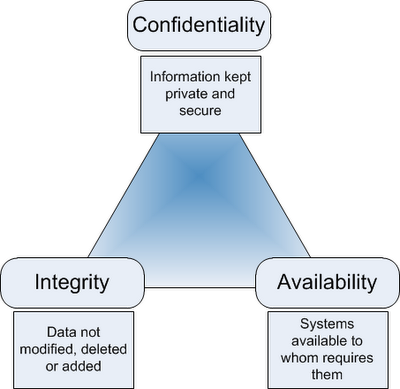
\includegraphics[width=.55\textwidth]{figuras/c-i-a.png}
  \caption[Elementos principales de seguridad de la información]{Elementos principales de seguridad de la información\\
  \footnotesize{Fuente: \textit{http://geraintw.blogspot.com.es/2012/09/cia-infosec.html}}}
  \label{fig:fundamentos-seguridad}
\end{figure}


\section*{Ejemplo de lista con números}

\begin{enumerate}

\item Confidencialidad:\\
El principio de confidencialidad consiste en asegurar que la información es accesible sólo para aquellos destinatarios que estén autorizados, con independencia de dónde se almacene la información.
La confidencialidad de los datos se implementa mediante mecanismos de control de acceso, tanto físicos (hardware) como  de programación (software).

\item Integridad:\\
La integridad de los datos se refiere a garantizar el estado de la información, protegiéndola de cambios accidentales o malintencionados. Mantener la integridad es esencial para la privacidad, la seguridad y la fiabilidad de los datos almacenados en un sistema.
Las medidas que se utilizan para mitigar posibles fallos en los datos incluyen: copias de seguridad regulares, almacenamiento seguro de esas copias fuera del lugar de trabajo y herramientas de control de integridad.

\item Disponibilidad:\\
La disponibilidad de los datos tiene como objetivo que los usuarios autorizados tengan acceso a la información en el momento que la necesiten. Esto implica garantizar el correcto funcionamiento de los equipos utilizados para almacenar y procesar los datos, de los controles de seguridad para protegerlos, y de los canales de comunicación utilizados para acceder a ellos.

\end{enumerate}


\section*{Una tabla con varias cabeceras}
\label{Ciberseguridad robótica}

La tabla~\ref{tabla1} extiende a los robots sociales y asistenciales la clasificación de criticidad para sistemas industriales, propuesta en \cite{CSSP}.

\begin{table*}[ht]
	\centering
	\caption{Perfiles de seguridad asociados a la robótica}
	\label{tabla1}
	\begin{tabular}{|l|ccc|}
		\cline{2-4}
		\multicolumn{1}{c}{} & \multicolumn{3}{|c|}{Criticidad} \\
		\cline{1-4}
		\multicolumn{1}{|c|}{Perfil} &  Confidencialidad & Integridad & Disponibilidad \\ \hline
		Estación de trabajo (PC) & Alta & Alta 	&  Baja \\
		Equipo para control industrial & Baja & Media & Muy alta \\
		Robots asistenciales & Muy alta & Muy alta & Muy alta \\
		Robots sociales & Muy alta & Media & Baja \\ \hline
	\end{tabular}
\end{table*}


\section*{Descripción de ROS: Robot Operating System}
\label{ROS}

Vistazo general sobre ROS:\\
- Historia y versión actual.\\
- Aplicación: investigación y también robots comerciales.\\
- Arquitectura: componentes básicos y funcionamiento.


\section*{Ejemplo de código fuente}

\vspace{0.5cm}  % Añado espacio vertical extra para separar el código del título de la sección.

\begin{lstlisting}
#!/bin/bash

# VARIABLES GLOBALES:

BASHRC_FILE="$HOME/.bashrc"
HOST_VAR_NAME="ROS_HOSTNAME"
MASTER_VAR_NAME="ROS_MASTER_URI"
ROS_PORT="11311"
HOST_IP=""    # Se asigna por parametro.
MASTER_IP=""  # Se asigna por parametro.
FILENAME="$(basename $0)"

# FUNCIONES:

description() {
if [ $1 -ne 0 ]; then
echo -e "\n  ========"
fi
echo -e "\n  This script adds or modifies $HOST_VAR_NAME and $MASTER_VAR_NAME variables"
echo -e "    in the '~/.bashrc' file of current user.\n"
}
\end{lstlisting}



%*********************************************

\chapter{Estudio del problema}
\label{Estudio del problema}

Se presenta el contexto de realización del trabajo realizando una revisión de las tecnologías, plataformas, herramientas o trabajos previos realizados en el mismo. Extensión aproximada de veinte páginas.

\section{El contexto del problema}

Breve descripción del contexto de realización del trabajo. Sirve para situar al lector.


\section{El estado de la cuestión}

Revisión de los trabajos existentes.

\section{La definición del problema}

Descripción del problema que ha motivado nuestro trabajo. Redactar en lenguaje sencillo y enumerando, de manera explícita, las limitaciones encontradas.

\chapter{Gestión de proyecto software}
\label{Gestión de proyecto software}

Realizar una simulación de la gestión del proyecto software desarrollo. La gestión simulará un proyecto real, realizado con las condiciones habituales del entorno empresarial. El objetivo del capítulo es plasmar los conocimientos adquiridos a lo largo de la titulación y no la forma en la cual se ha gestionado el Trabajo Fin de Máster. Extensión máxima de veinte páginas.

\section{Alcance del proyecto}
\label{Alcance del proyecto}

\subsection{Definición del proyecto}

\subsection{Estimación de tareas y recursos}

\subsection{Presupuesto}

A continuación se detalla un presupuesto estimado para el coste total de este proyecto.

\subsubsection{Coste de personal}

\begin{table*}[ht]
	\centering
	\caption{Presupuesto de personal}
	\label{tabla2}
	\makebox[\textwidth]{  % Para centrar una tabla más ancha que la página definida.
		\begin{tabular}{|c|c|c|c|c|}
			\cline{1-5}
			Tarea &	Perfil & Horas & Euros/Hora  &  Total\\ \hline
			Desarrollo aplicación &	Programador Junior & 80 & 60 & 4800 \euro\\
			Integración en entorno robótico & Programador Senior & 20 & 100 & 2000 \euro\\
			Pruebas & Ingeniero de Pruebas & 20 & 80 & 1600 \euro\\
			Supervisión del Proyecto & Jefe de Proyecto & 10 & 120 & 1200 \euro\\ \hline\hline
			\multicolumn{4}{|c|}{Total} & \multicolumn{1}{c|}{10100 \euro}\\ \hline
		\end{tabular}
	}
\end{table*}


\subsubsection{Coste del hardware}

Para la realización de este proyecto se ha realizado la compra de:

\begin{enumerate}
	
	\item Ordenador con Intel i7:
	
	Placa base: MSI GE62 6QF-060ES Heroes Ed.
	
	Procesador: Intel i7-6700HQ
	
	RAM: 16 GB
	
	Disco duro: 1TB + 128GB SSD
	
	Tarjeta gráfica: Nvidia GTX970M
	
	Monitor: 15.6"
	
	\begin{itemize}
		\item Precio (sin IVA): 986,71 \euro\\
	\end{itemize}
	
	\item Ordenador con Intel Atom:
	
	Asus Transformer Book H100TAM DK028B
	
	RAM: 32GB
	
	Disco duro: 500GB
	
	\begin{itemize}
		\item Precio (sin IVA): 260,27 \euro
	\end{itemize}
	
\end{enumerate}


\subsubsection{Coste total}

\begin{table*}[ht]
	\centering
	\caption{Presupuesto total}
	\label{tabla3}
	\makebox[\textwidth]{  % Para centrar una tabla ancha.
		\begin{tabular}{|l|l|}
			\cline{1-2}
			Concepto &	Coste (Euros) \\ \hline
			Costes de personal & 10100  \\
			Costes de hardware  & 1246,98   \\ \hline
			Subtotal  &  11346,97 \\
			IVA (21\%) & 2882,86 \\ \hline \hline
			Total Proyecto & \textbf{13729,83 \euro} \\ \hline
	\end{tabular}}
\end{table*}

\section{Plan de trabajo}
\label{Plan de trabajo}


\subsection{Identificación de tareas}

\subsection{Estimación de tareas}

\subsection{Planificación de tareas}



\section{Gestión de recursos}

\subsection{Especificación de recursos}

\subsection{Asignación de recursos}




\section{Gestión de riesgos}

\subsection{Identificación de riesgos}

\subsection{Análisis de riesgos}



\chapter{Solución}
\label{Solución}

Explicación de la solución llevada a cabo. Si se trata de un desarrollo se incidirá en el proceso de desarrollo; en otro caso, se justificará y describirá la solución propuesta. El capítulo tendrá una extensión aproximada de cuarenta páginas y, en ningún caso, excederá las cincuenta.

\section{Descripción de la solución}

Breve descripción del tipo de solución adoptada: si es una aplicación y qué características tiene, si se trata de un tutorial, un modelo, etc.


\section{El proceso de desarrollo}

Explicar el modelo de proceso y la estructura de la sección.

\subsection{Análisis}

Fase de análisis


\subsubsection{Definición de requisitos}

Enumerar los requisitos del sistema dividiéndoles en funcionales y no funcionales.

\subsubsection{Especificación de requisitos}

Analizar y especificar los requisitos desde el punto de vista del comportamiento, estructura y funcionalidad del sistema.


\subsection{Diseño}

Fase de diseño

\subsubsection{Diseño de sistema}

Se expone la ARQUITECTURA del sistema y las TECNOLOGÍAS utilizadas en el desarrollo.

\subsubsection{Diseño detallado}

Se describe el diseño de las capas de PERSISTENCIA, MODELO e INTERFAZ del sistema.


\subsection{Implementación}

Hablar de las HERRAMIENTAS utilizadas durante el desarrollo, la ORGANIZACIÓN del proyecto y aquellas peculiaridades de la forma de implementación.

\subsection{Pruebas}

Centrarse en pruebas unitarias (no incluir todas las pruebas sino informes de las mismas) y de sistema (mostrar que cumple los casos de uso).


\section{El producto del desarrollo}

En el caso de desarrollar una herramienta es necesario mostrar, brevemente, el tipo de herramienta generada. Incluir algún pantallazo de la herramienta, su funcionalidad y la forma de ejecución de la misma.

\chapter{Evaluación}
\label{Evaluación}


Demostración de la validez de la solución elaborada. La solución se considera válida si resuelve los problemas expuestos en el planteamiento del problema y satisface los objetivos definidos en la introducción. Según el caso la forma de evaluación se basará en la ejecución de casos de prueba o en la realización de cuestionarios. Extensión entre quince y veinte páginas.

\section{Proceso de evaluación}

\subsection{Forma de evaluación}

Explicar la forma en la cual se ha evaluado la aplicación

\subsection{Casos de prueba}

Casos de pruebas realizados

\section{Análisis de resultados}



\mychapter{1}{Conclusión}

Expresión personal del conjunto de conclusiones que, a juicio del autor, se derivan de los resultados expuestos en el trabajo.Deberá tener una extensión entre cinco y diez páginas.

\subsection*{Aportaciones realizadas}



\subsection*{Trabajos futuros}



\subsection*{Problemas encontrados}



\section*{Opiniones personales}



%%%% BIBLIOGRAFÍA %%%%
\bibliographystyle{splncs.bst}  % Fichero con el formato de la bibliografía.

\renewcommand\bibname{Lista de referencias}

%\bibliography{Refs-proyecto}    % Fichero con las referencias.
Información bibliográfica citada en el texto del trabajo. Otras lecturas recomendadas o consultadas, de figurar, aparecerán en anexos.
Se debe seguir la norma ISO 690 (buscar en google ISO 690 ugr)

% También se puede optar por incluir las referencias desde aquí mismo:
\begin{thebibliography}{1}
	
\bibitem{uno} \textit P. V. Nikitin, K. V. S. Rao y S. Lazar, ``An overview of near field UHF RFID", IEEE RFID. Conferencia, 2007, p\'ags.167-174.
\bibitem{dos} \textit M. M. Singh, K. A. A. K. Adzman, y R. Hassan, ``Near Field Communication (NFC) Technology Security Vulnerabilities and Countermeasures", International Journal of Engineering \& Technology Vol.7, N\textdegree 4.31, p\'ags.298-305, 2018.
\bibitem{tres} \textit ISO/IEC 18092. ``Near Field Comunication: interface and protocolo", 2004.
\bibitem{cuatro} \textit ECMA International (2005). ``Near Field Communication - White Paper”, Ecma/TC32-TG19/2005/ 012, Internet: www.ecma international.org, 2005.
\bibitem{cinco} \textit ``NFC Data Exchange Format (NDEF), NFC Forum Technical Specification"
\bibitem{seis} \textit ``NFC-Near Field Communication, Reader/Writer Operating Mode”
\bibitem{siete} \textit F. Fahrianto, M. F. Lubis, and A. Fiade, ``Denial-of-service attack possibilities on NFC technology”, 2016 4th International Conference on Cyber and IT Service Management, IEEE, págs.1-5, 2016
\bibitem{ocho} \textit H. Eun, H. Lee, and H. Oh, ``Conditional privacy preserving security protocol for NFC applications”, IEEE T. Cons. Electr., Vol.59, N\textdegree.1, págs.153-160, 2013

\bibitem{CSSP}
{CSSP, D.}:
\newblock \textit{Recommended Practice: Improving Industrial Control Systems
  Cybersecurity with Defense-In-Depth Strategies}.
\newblock US-CERT Defense In Depth. (Octubre 2009)

\end{thebibliography}



%%%% ANEXOS %%%%
\renewcommand{\appendixname}{Anexo}
\appendix

\chapter{Control de versiones}
\label{Control de versiones}




\chapter{Seguimiento de proyecto fin de máster}
\label{Seguimiento de proyecto fin de máster}


Obligatorio. Seguimiento del trabajo real.

\section{Forma de seguimiento}

\section{Planificación inicial}

\section{Planificación final}
Si el trabajo ha consistido en la elaboración de una aplicación se incluirá el manual de usuario de la misma.


\chapter{Cuestionario de evaluación}
\label{Cuestionario de evaluación}

Cuestionarios utilizados durante la fase de evaluación.



\end{document}
